\documentclass{beamer}
\usepackage{tikz-network}
\usepackage[table]{xcolor}
\title{Graph Theory}
\begin{document}
\begin{frame}
\frametitle{Initial Graph}
\begin{center}
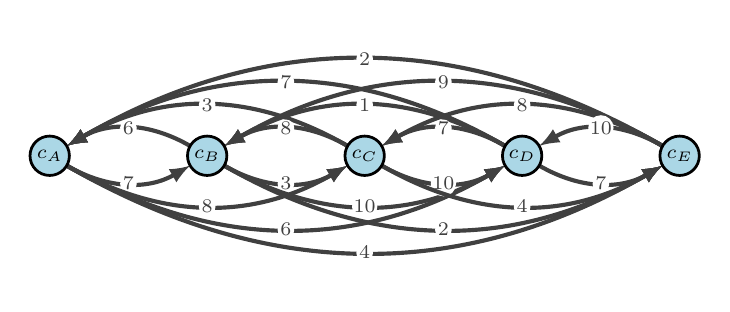
\begin{tikzpicture}
 \Vertex[x=0, y=0, size=0.5, label=$c_A$]{A}
 \Vertex[x=2, y=0, size=0.5, label=$c_B$]{B}
 \Vertex[x=4, y=0, size=0.5, label=$c_C$]{C}
 \Vertex[x=6, y=0, size=0.5, label=$c_D$]{D}
 \Vertex[x=8, y=0, size=0.5, label=$c_E$]{E}
 
 \Edge[bend=-30, label=$7$, Direct](A)(B) 
 \Edge[bend=-30, label=$8$, Direct](A)(C) 
 \Edge[bend=-30, label=$6$, Direct](A)(D) 
 \Edge[bend=-30, label=$4$, Direct](A)(E) 
 \Edge[bend=-30, label=$6$, Direct](B)(A) 
 \Edge[bend=-30, label=$3$, Direct](B)(C) 
 \Edge[bend=-30, label=$10$, Direct](B)(D) 
 \Edge[bend=-30, label=$2$, Direct](B)(E) 
 \Edge[bend=-30, label=$3$, Direct](C)(A) 
 \Edge[bend=-30, label=$8$, Direct](C)(B) 
 \Edge[bend=-30, label=$10$, Direct](C)(D) 
 \Edge[bend=-30, label=$4$, Direct](C)(E) 
 \Edge[bend=-30, label=$7$, Direct](D)(A) 
 \Edge[bend=-30, label=$1$, Direct](D)(B) 
 \Edge[bend=-30, label=$7$, Direct](D)(C) 
 \Edge[bend=-30, label=$7$, Direct](D)(E) 
 \Edge[bend=-30, label=$2$, Direct](E)(A) 
 \Edge[bend=-30, label=$9$, Direct](E)(B) 
 \Edge[bend=-30, label=$8$, Direct](E)(C) 
 \Edge[bend=-30, label=$10$, Direct](E)(D)\end{tikzpicture}
\end{center}
\end{frame}



\begin{frame}
\frametitle{Table D$_{0}$}
\begin{center}
    \begin{tabular}{|c||c|c|c|c|c|}
        \hline
        \textbf{D} & \textbf{0} & \textbf{1} & \textbf{2} & \textbf{3} & \textbf{4} \\
        \hline
        \hline
        \textbf{0}& 4 & 7 & 8 & 6 & 4 \\
        \hline
        \textbf{1}& 6 & 7 & 3 & 10 & 2 \\
        \hline
        \textbf{2}& 3 & 8 & 1 & 10 & 4 \\
        \hline
        \textbf{3}& 7 & 1 & 7 & 3 & 7 \\
        \hline
        \textbf{4}& 2 & 9 & 8 & 10 & 3 \\
        \hline
    \end{tabular}
\end{center}


\end{frame}


\begin{frame}
\frametitle{Table P$_{0}$}
\begin{center}
    \begin{tabular}{|c||c|c|c|c|c|}
        \hline
        \textbf{P} & \textbf{0} & \textbf{1} & \textbf{2} & \textbf{3} & \textbf{4} \\
        \hline
        \hline
        \textbf{0}& 0 & 0 & 0 & 0 & 0 \\
        \hline
        \textbf{1}& 0 & 0 & 0 & 0 & 0 \\
        \hline
        \textbf{2}& 0 & 0 & 0 & 0 & 0 \\
        \hline
        \textbf{3}& 0 & 0 & 0 & 0 & 0 \\
        \hline
        \textbf{4}& 0 & 0 & 0 & 0 & 0 \\
        \hline
    \end{tabular}
\end{center}


\end{frame}


\begin{frame}
\frametitle{Table D$_{1}$}
\begin{center}
    \begin{tabular}{|c||c|c|c|c|c|}
        \hline
        \textbf{D} & \textbf{0} & \textbf{1} & \textbf{2} & \textbf{3} & \textbf{4} \\
        \hline
        \hline
        \textbf{0}& 4 & 7 & 8 & 6 & 4 \\
        \hline
        \textbf{1}& 6 & 7 & 3 & 10 & 2 \\
        \hline
        \textbf{2}& 3 & 8 & 1 & \cellcolor{yellow}9 & 4 \\
        \hline
        \textbf{3}& 7 & 1 & 7 & 3 & 7 \\
        \hline
        \textbf{4}& 2 & 9 & 8 & \cellcolor{yellow}8 & 3 \\
        \hline
    \end{tabular}
\end{center}


\end{frame}


\begin{frame}
\frametitle{Table P$_{1}$}
\begin{center}
    \begin{tabular}{|c||c|c|c|c|c|}
        \hline
        \textbf{P} & \textbf{0} & \textbf{1} & \textbf{2} & \textbf{3} & \textbf{4} \\
        \hline
        \hline
        \textbf{0}& 0 & 0 & 0 & 0 & 0 \\
        \hline
        \textbf{1}& 0 & 0 & 0 & 0 & 0 \\
        \hline
        \textbf{2}& 0 & 0 & 0 & \cellcolor{yellow}0 & 0 \\
        \hline
        \textbf{3}& 0 & 0 & 0 & 0 & 0 \\
        \hline
        \textbf{4}& 0 & 0 & 0 & \cellcolor{yellow}0 & 0 \\
        \hline
    \end{tabular}
\end{center}


\end{frame}


\begin{frame}
\frametitle{Table D$_{2}$}
\begin{center}
    \begin{tabular}{|c||c|c|c|c|c|}
        \hline
        \textbf{D} & \textbf{0} & \textbf{1} & \textbf{2} & \textbf{3} & \textbf{4} \\
        \hline
        \hline
        \textbf{0}& 4 & 7 & 8 & 6 & 4 \\
        \hline
        \textbf{1}& 6 & 7 & 3 & 10 & 2 \\
        \hline
        \textbf{2}& 3 & 8 & 1 & 9 & 4 \\
        \hline
        \textbf{3}& 7 & 1 & \cellcolor{yellow}4 & 3 & \cellcolor{yellow}3 \\
        \hline
        \textbf{4}& 2 & 9 & 8 & 8 & 3 \\
        \hline
    \end{tabular}
\end{center}


\end{frame}


\begin{frame}
\frametitle{Table P$_{2}$}
\begin{center}
    \begin{tabular}{|c||c|c|c|c|c|}
        \hline
        \textbf{P} & \textbf{0} & \textbf{1} & \textbf{2} & \textbf{3} & \textbf{4} \\
        \hline
        \hline
        \textbf{0}& 0 & 0 & 0 & 0 & 0 \\
        \hline
        \textbf{1}& 0 & 0 & 0 & 0 & 0 \\
        \hline
        \textbf{2}& 0 & 0 & 0 & 0 & 0 \\
        \hline
        \textbf{3}& 0 & 0 & \cellcolor{yellow}1 & 0 & \cellcolor{yellow}1 \\
        \hline
        \textbf{4}& 0 & 0 & 0 & 0 & 0 \\
        \hline
    \end{tabular}
\end{center}


\end{frame}


\begin{frame}
\frametitle{Table D$_{3}$}
\begin{center}
    \begin{tabular}{|c||c|c|c|c|c|}
        \hline
        \textbf{D} & \textbf{0} & \textbf{1} & \textbf{2} & \textbf{3} & \textbf{4} \\
        \hline
        \hline
        \textbf{0}& 4 & 7 & 8 & 6 & 4 \\
        \hline
        \textbf{1}& 6 & 7 & 3 & 10 & 2 \\
        \hline
        \textbf{2}& 3 & 8 & 1 & 9 & 4 \\
        \hline
        \textbf{3}& 7 & 1 & 4 & 3 & 3 \\
        \hline
        \textbf{4}& 2 & 9 & 8 & 8 & 3 \\
        \hline
    \end{tabular}
\end{center}


\end{frame}


\begin{frame}
\frametitle{Table P$_{3}$}
\begin{center}
    \begin{tabular}{|c||c|c|c|c|c|}
        \hline
        \textbf{P} & \textbf{0} & \textbf{1} & \textbf{2} & \textbf{3} & \textbf{4} \\
        \hline
        \hline
        \textbf{0}& 0 & 0 & 0 & 0 & 0 \\
        \hline
        \textbf{1}& 0 & 0 & 0 & 0 & 0 \\
        \hline
        \textbf{2}& 0 & 0 & 0 & 0 & 0 \\
        \hline
        \textbf{3}& 0 & 0 & 1 & 0 & 1 \\
        \hline
        \textbf{4}& 0 & 0 & 0 & 0 & 0 \\
        \hline
    \end{tabular}
\end{center}


\end{frame}


\begin{frame}
\frametitle{Table D$_{4}$}
\begin{center}
    \begin{tabular}{|c||c|c|c|c|c|}
        \hline
        \textbf{D} & \textbf{0} & \textbf{1} & \textbf{2} & \textbf{3} & \textbf{4} \\
        \hline
        \hline
        \textbf{0}& 4 & 7 & 8 & 6 & 4 \\
        \hline
        \textbf{1}& 6 & 7 & 3 & 10 & 2 \\
        \hline
        \textbf{2}& 3 & 8 & 1 & 9 & 4 \\
        \hline
        \textbf{3}& 7 & 1 & 4 & 3 & 3 \\
        \hline
        \textbf{4}& 2 & 9 & 8 & 8 & 3 \\
        \hline
    \end{tabular}
\end{center}


\end{frame}


\begin{frame}
\frametitle{Table P$_{4}$}
\begin{center}
    \begin{tabular}{|c||c|c|c|c|c|}
        \hline
        \textbf{P} & \textbf{0} & \textbf{1} & \textbf{2} & \textbf{3} & \textbf{4} \\
        \hline
        \hline
        \textbf{0}& 0 & 0 & 0 & 0 & 0 \\
        \hline
        \textbf{1}& 0 & 0 & 0 & 0 & 0 \\
        \hline
        \textbf{2}& 0 & 0 & 0 & 0 & 0 \\
        \hline
        \textbf{3}& 0 & 0 & 1 & 0 & 1 \\
        \hline
        \textbf{4}& 0 & 0 & 0 & 0 & 0 \\
        \hline
    \end{tabular}
\end{center}


\end{frame}


\begin{frame}
\frametitle{Table D$_{5}$}
\begin{center}
    \begin{tabular}{|c||c|c|c|c|c|}
        \hline
        \textbf{D} & \textbf{0} & \textbf{1} & \textbf{2} & \textbf{3} & \textbf{4} \\
        \hline
        \hline
        \textbf{0}& 4 & 7 & 8 & 6 & 4 \\
        \hline
        \textbf{1}& \cellcolor{yellow}4 & 7 & 3 & 10 & 2 \\
        \hline
        \textbf{2}& 3 & 8 & 1 & 9 & 4 \\
        \hline
        \textbf{3}& \cellcolor{yellow}5 & 1 & 4 & 3 & 3 \\
        \hline
        \textbf{4}& 2 & 9 & 8 & 8 & 3 \\
        \hline
    \end{tabular}
\end{center}


\end{frame}


\begin{frame}
\frametitle{Table P$_{5}$}
\begin{center}
    \begin{tabular}{|c||c|c|c|c|c|}
        \hline
        \textbf{P} & \textbf{0} & \textbf{1} & \textbf{2} & \textbf{3} & \textbf{4} \\
        \hline
        \hline
        \textbf{0}& 0 & 0 & 0 & 0 & 0 \\
        \hline
        \textbf{1}& \cellcolor{yellow}4 & 0 & 0 & 0 & 0 \\
        \hline
        \textbf{2}& 0 & 0 & 0 & 0 & 0 \\
        \hline
        \textbf{3}& \cellcolor{yellow}4 & 0 & 1 & 0 & 1 \\
        \hline
        \textbf{4}& 0 & 0 & 0 & 0 & 0 \\
        \hline
    \end{tabular}
\end{center}


\end{frame}\begin{frame}
\frametitle{Final Graph}
\begin{center}
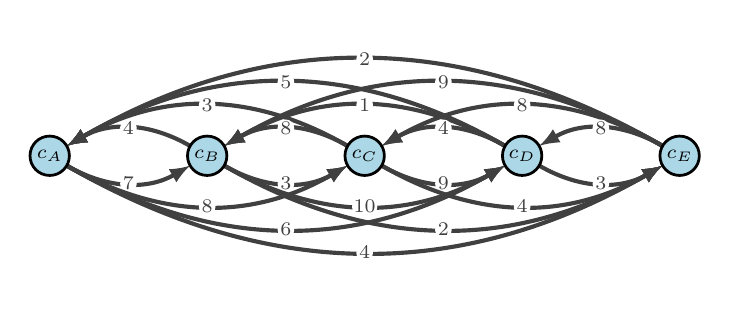
\begin{tikzpicture}
 \Vertex[x=0, y=0, size=0.5, label=$c_A$]{A}
 \Vertex[x=2, y=0, size=0.5, label=$c_B$]{B}
 \Vertex[x=4, y=0, size=0.5, label=$c_C$]{C}
 \Vertex[x=6, y=0, size=0.5, label=$c_D$]{D}
 \Vertex[x=8, y=0, size=0.5, label=$c_E$]{E}
 
 \Edge[bend=-30, label=$7$, Direct](A)(B) 
 \Edge[bend=-30, label=$8$, Direct](A)(C) 
 \Edge[bend=-30, label=$6$, Direct](A)(D) 
 \Edge[bend=-30, label=$4$, Direct](A)(E) 
 \Edge[bend=-30, label=$4$, Direct](B)(A) 
 \Edge[bend=-30, label=$3$, Direct](B)(C) 
 \Edge[bend=-30, label=$10$, Direct](B)(D) 
 \Edge[bend=-30, label=$2$, Direct](B)(E) 
 \Edge[bend=-30, label=$3$, Direct](C)(A) 
 \Edge[bend=-30, label=$8$, Direct](C)(B) 
 \Edge[bend=-30, label=$9$, Direct](C)(D) 
 \Edge[bend=-30, label=$4$, Direct](C)(E) 
 \Edge[bend=-30, label=$5$, Direct](D)(A) 
 \Edge[bend=-30, label=$1$, Direct](D)(B) 
 \Edge[bend=-30, label=$4$, Direct](D)(C) 
 \Edge[bend=-30, label=$3$, Direct](D)(E) 
 \Edge[bend=-30, label=$2$, Direct](E)(A) 
 \Edge[bend=-30, label=$9$, Direct](E)(B) 
 \Edge[bend=-30, label=$8$, Direct](E)(C) 
 \Edge[bend=-30, label=$8$, Direct](E)(D)\end{tikzpicture}
\end{center}
\end{frame}
\end{document}
